\documentclass[12pt,letterpaper]{article}
\usepackage[utf8]{inputenc}
\usepackage[spanish]{babel}
\usepackage{graphicx}
\usepackage[left=2cm,right=2cm,top=2cm,bottom=2cm]{geometry}
\usepackage{graphicx} % figuras
% \usepackage{subfigure} % subfiguras
\usepackage{float} % para usar [H]
\usepackage{amsmath}
%\usepackage{txfonts}
\usepackage{stackrel} 
\usepackage{multirow}
\usepackage{enumerate} % enumerados

\usepackage{hyperref}


\renewcommand{\labelitemi}{$-$}
\renewcommand{\labelitemii}{$\cdot$}
% \author{}
% \title{Caratula}
\begin{document}

% Fancy Header and Footer
% \usepackage{fancyhdr}
% \pagestyle{fancy}
% \cfoot{}
% \rfoot{\thepage}
%

% \usepackage[hidelinks]{hyperref} % CREA HYPERVINCULOS EN INDICE

% \author{}
\title{Caratula}

\begin{titlepage}
\begin{center}
\large{UNIVERSIDAD PRIVADA DE TACNA}\\
\vspace*{-0.025in}
\begin{figure}[htb]
\begin{center}

\includegraphics[width=8cm]{./Imagenes/logo}
\end{center}
\end{figure}
\vspace*{0.15in}
INGENIERIA DE SISTEMAS  \\

\vspace*{0.5in}
\begin{large}
TITULO:\\
\end{large}

\vspace*{0.1in}
\begin{Large}
\textbf{INFORME DE LABORATORIO No 02} \\
\end{Large}

\vspace*{0.3in}
\begin{Large}
\textbf{CURSO:} \\
\end{Large}

\vspace*{0.1in}
\begin{large}
INTELIGENCIA DE NEGOCIOS\\
\end{large}

\vspace*{0.3in}
\begin{Large}
\textbf{DOCENTE(ING):} \\
\end{Large}

\vspace*{0.1in}
\begin{large}
 Patrick Cuadros Quiroga\\
\end{large}

\vspace*{0.2in}
\vspace*{0.1in}
\begin{large}
Integrantes: \\
\begin{flushleft}


Quispe Mamani Angelo        \hfill	(2015052826) \\

\end{flushleft}
\end{large}
\end{center}

\end{titlepage}


\tableofcontents % INDICE
\thispagestyle{empty} % INDICE SIN NUMERO
\newpage
\setcounter{page}{1} % REINICIAR CONTADOR DE PAGINAS DESPUES DEL INDICE

\section{Desarrollo } 

\begin{itemize}



\item Desarollo de Tarea1 del Laboratorio 2 de PowerBI
\begin{center}
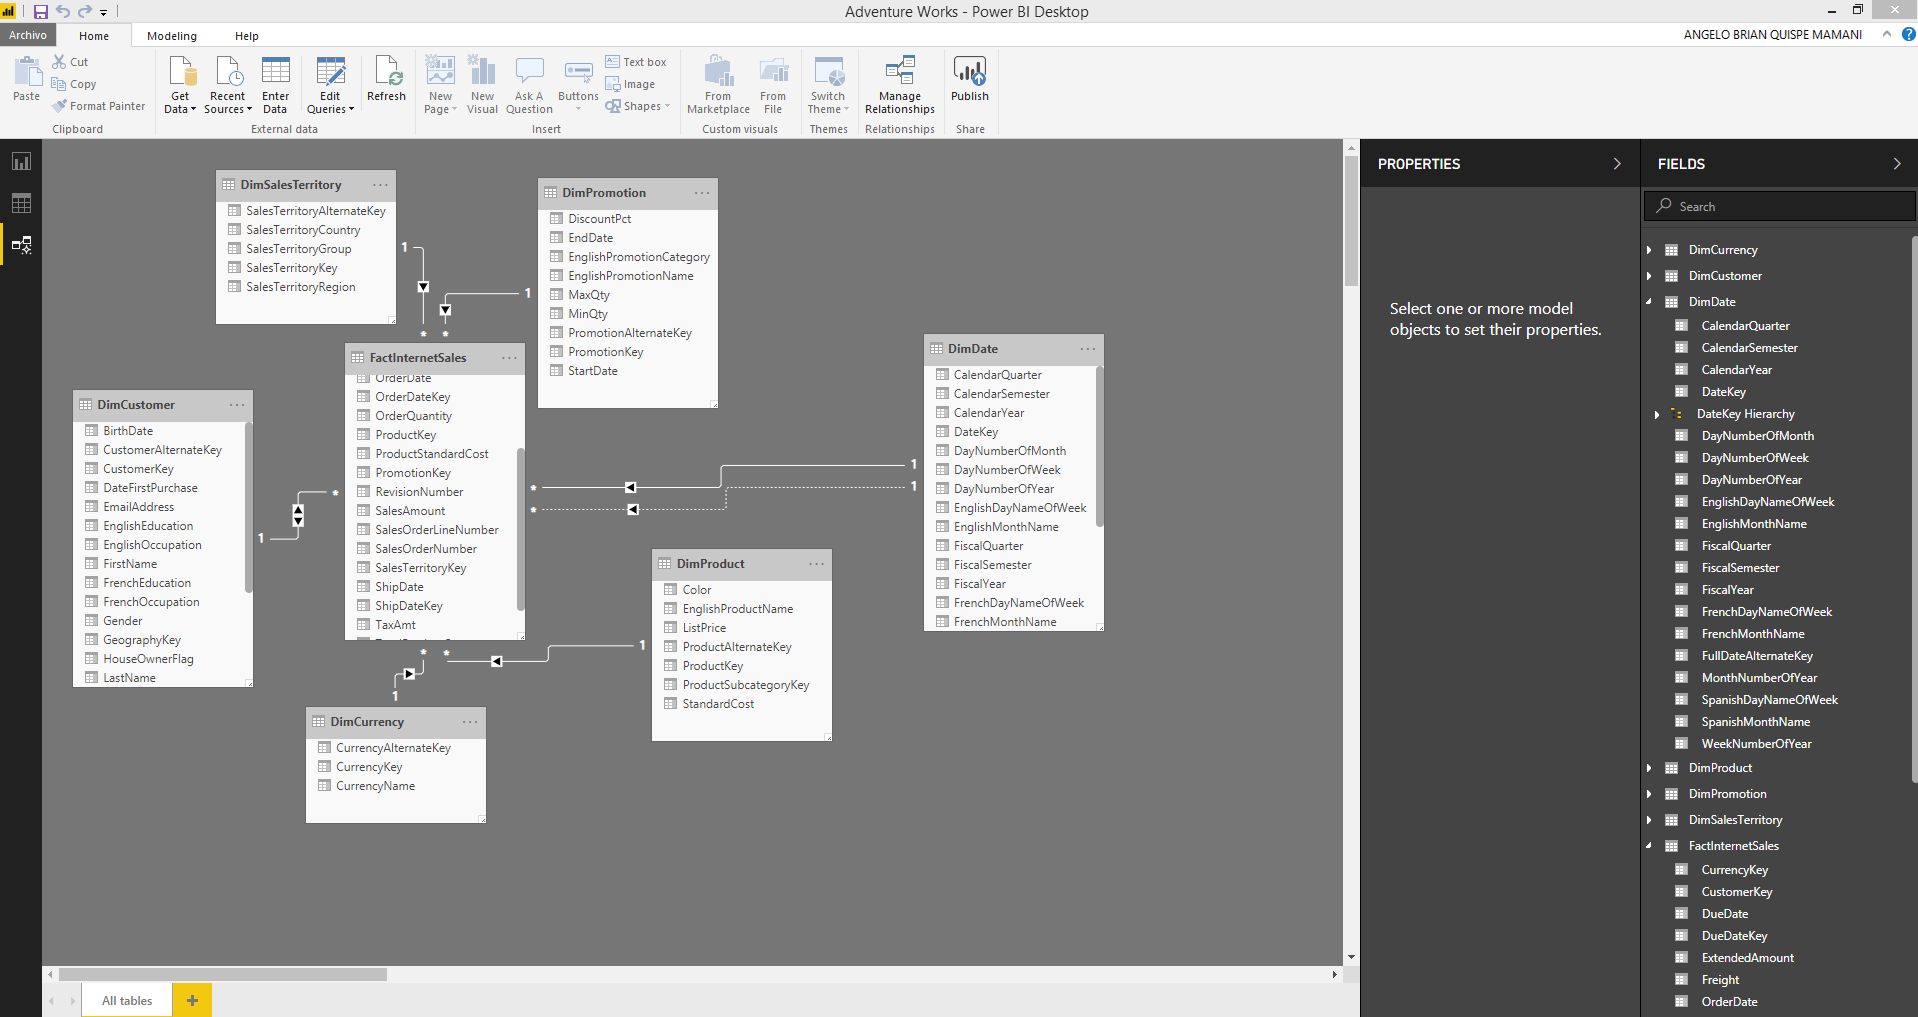
\includegraphics[scale=0.30]{./Imagenes/1.png}
\end{center}


\item Desarollo de Tarea2 del Laboratorio 2 de PowerBI
\begin{center}
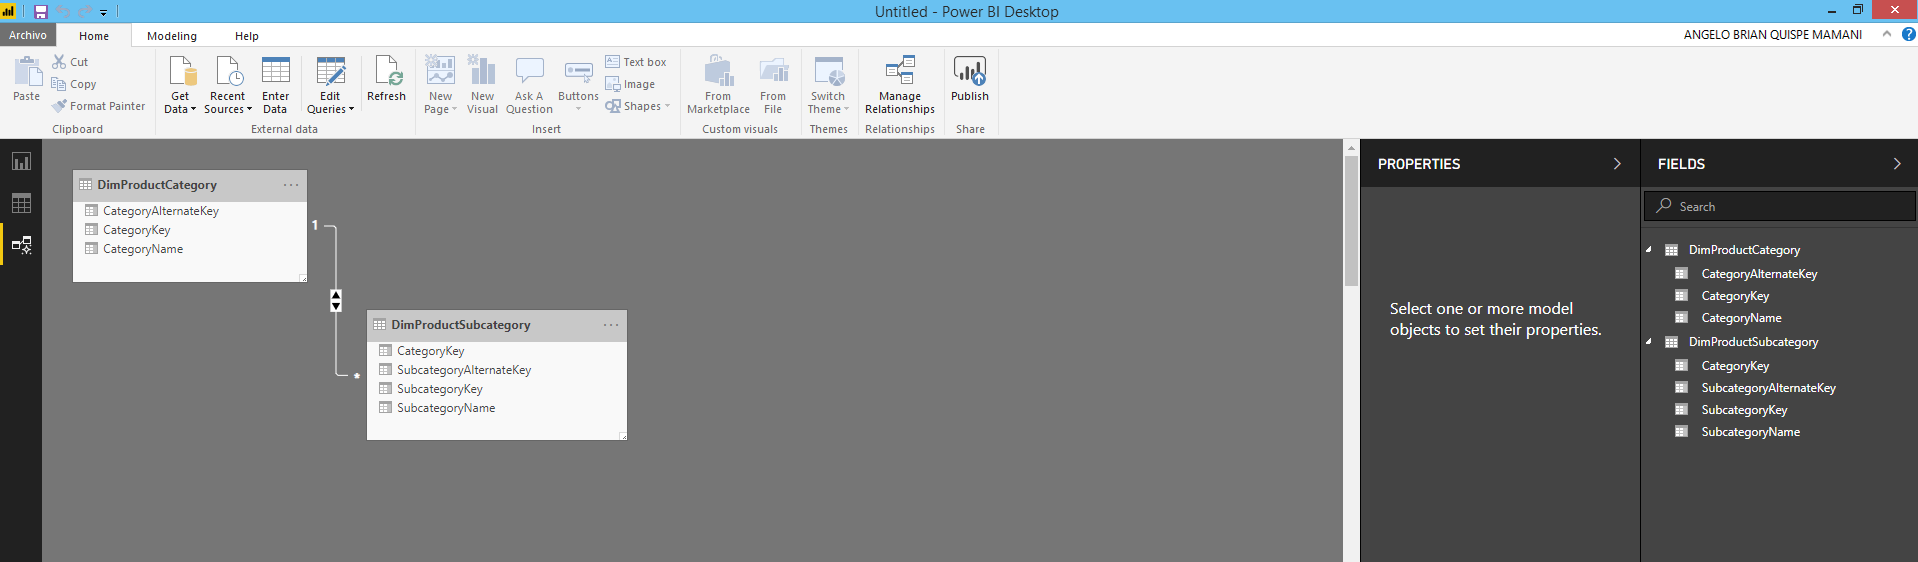
\includegraphics[scale=0.30]{./Imagenes/2.png}
\end{center}


\item Desarollo de Consultas del Laboratorio 2 de PowerBI
\begin{center}
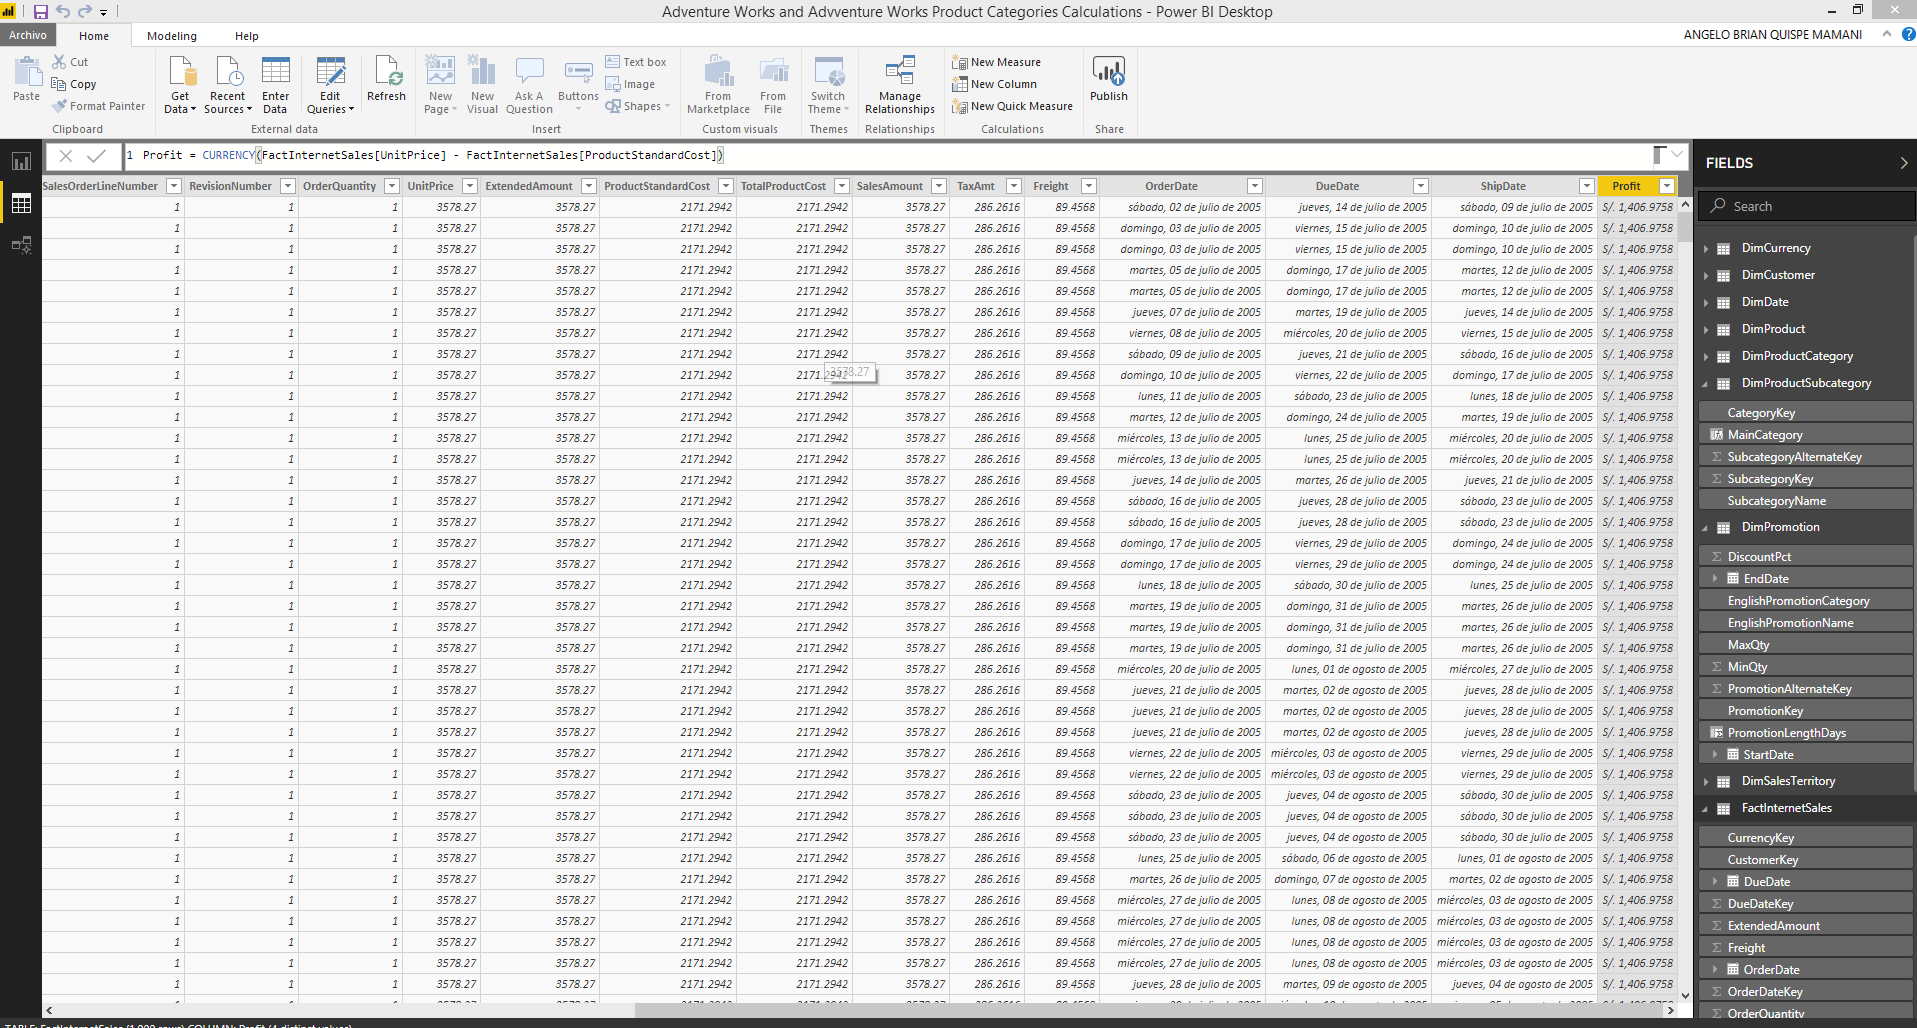
\includegraphics[scale=0.30]{./Imagenes/3.png}
\end{center}



\item Direccion de la Tarea1 en PowerBI

\begin{center}
\href{https://app.powerbi.com/groups/me/reports/a18217bf-4119-48fe-bb0c-889bd8766287?ctid=b6b466ee-468d-4011-b9fc-fbdcf82ac90a}{https://app.powerbi.com/groups/me/reports/a18217bf-4119-48fe-bb0c-889bd8766287?ctid=b6b466ee-468d-4011-b9fc-fbdcf82ac90a}
\end{center}


\item Direccion de la Tarea2 en PowerBI

\begin{center}
\href{https://app.powerbi.com/groups/me/reports/8a7d6c00-a7c4-4aaa-9708-912d70e525cb?ctid=b6b466ee-468d-4011-b9fc-fbdcf82ac90a}{https://app.powerbi.com/groups/me/reports/8a7d6c00-a7c4-4aaa-9708-912d70e525cb?ctid=b6b466ee-468d-4011-b9fc-fbdcf82ac90a}
\end{center}


\item Direccion de las Consultas en PowerBI

\begin{center}
\href{https://app.powerbi.com/groups/me/reports/67a36cce-b73b-47dc-a23b-b65b81d1863f?ctid=b6b466ee-468d-4011-b9fc-fbdcf82ac90a}{https://app.powerbi.com/groups/me/reports/67a36cce-b73b-47dc-a23b-b65b81d1863f?ctid=b6b466ee-468d-4011-b9fc-fbdcf82ac90a}
\end{center}




\end{itemize}







 	 	


\end{document}
